\section{Setup}
\label{sec:setup}

\subsection{Hardware}
% TODO: Describe the robot we are designing for
% TODO: Describe the sensors available
% TODO: Describe that we assume the robot to have some sort of communication method

For this project a differential drive robot with camera, lidar, odometry and communication capabilities is assumed. Lidar and odometry are used for localization using AMCL as discussed later ({\color{red} DISCUSS THIS}), the camera is used to look for the search object and a global communication channel is needed for the robots to share data. To get realistic parameters and to make use of ready made 3D models, URDF files and robot parameters, the Turtlebot 4 \cite{tb4} was chosen as the target platform. It is, however, important to note that the software developed in this project will run on any robot satisfying the sensor and communication requirements by changing the parameters to match in the source code. The Turtlebot has all the required hardware apart from a {\color{red} designated communication unit}. As this project focuses on simulation, the simulator will be responsible for passing messages between robots as they are sent. The software implementation is therefore {\color{red} communication method agnostic} as long as the messages the robots send are received by the other robots.

% TODO: Maybe mark the sensors on the robot
\begin{figure}[h]
    \begin{center}
        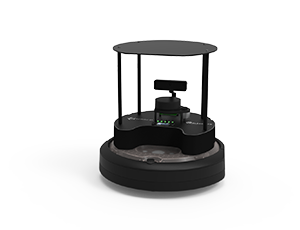
\includegraphics[width=0.55\textwidth]{figures/tb4.png}
    \end{center}
    \caption{Turtlebot 4}\label{fig:tb4}
\end{figure}



\section{Software Structure}
% TODO: Find a home for this figure
% TODO: Find a nice color scheme
% TODO: Refer to this figure in the text
\begin{figure}
    \begin{center}
        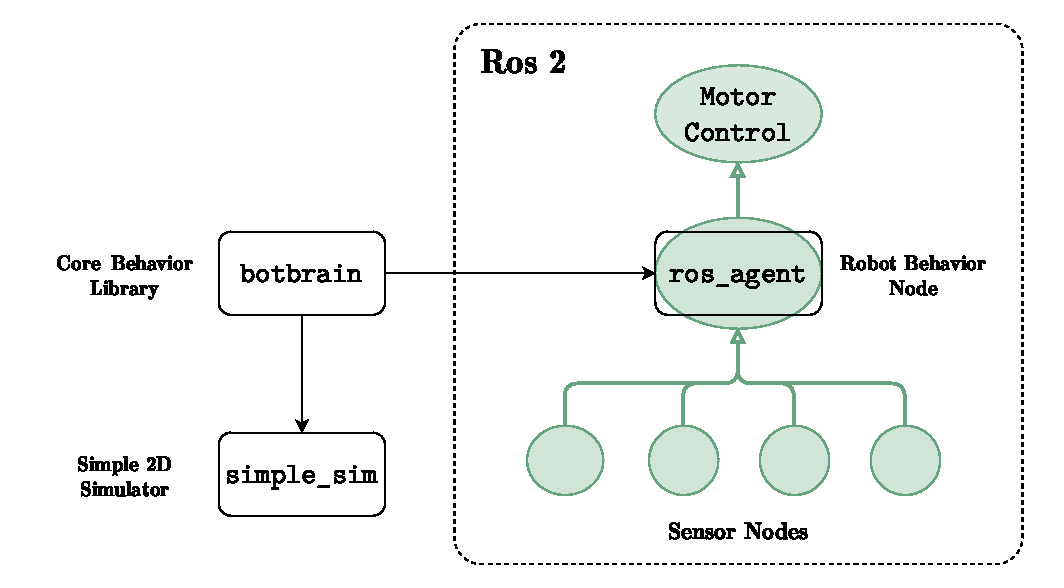
\includegraphics[width=0.95\textwidth]{figures/software-structure.pdf}
    \end{center}
    \caption{Software structure of the project. Black arrows indicate a library dependency and green arrows denote ROS 2 communication through topics. Square boxes are Rust crates while green circles are Ros 2 nodes. Notice that the core library \texttt{botbrain} is not part of the Ros 2 dependent code. It can therefore be used by the simple simulator without Ros 2.}\label{fig:}
\end{figure}


The software is divided into three main parts, the robot behavior implementation, a simple custom 2D
simulator, and a ROS 2 environment.

\subsection{Robot Behavior}
The robot behaviors are implemented in the botbrain rust crate. This crate defines the Robot interface
which is the only way for outside crates to interact with a robot’s internal state (see \cref{fig:robot-interface}).

\begin{figure}[H]
    \begin{center}
        \begin{minted}[autogobble]{rust}
            pub trait Robot {
                fn set_id(&mut self, id: RobotId);            // Set the id of the robot
                fn set_map(&mut self, world: Map); // The world the robot is operating in

                fn input_pose(&mut self, pose: RobotPose);    // Input the angle of the robot
                fn input_cam(&mut self, cam: CamData);        // Input data from the camera
                fn input_lidar(&mut self, lidar: LidarData);  // Input data from the lidar
                fn input_msgs(&mut self, msgs: Vec<Message>); // Input messages from other robots

                fn get_id(&self) -> &RobotId;                 // Get the id of the robot
                ...
            }
        \end{minted}
    \end{center}
    \caption{Methods of the \texttt{Robot} interface.}\label{fig:robot-interface}
\end{figure}

Interface methods prefixed with \texttt{set} are used to set up the internal state of the robot and should be called after creating a robot and before any other methods. The \texttt{input} prefix is used in functions which should be called as often as possible to update the world view of the robot. \texttt{get}-methods do not change the state of the robot and may be called at any time. Notice that there is no method which "runs" the robot to generate a control signal. This is because a \texttt{Robot} only represents the robot state, not the algorithm which uses that state to generate a control output. To generate a control output, the dynamic \texttt{Robot} must be passed to a behavior function as defined in \cref{fig:behavior-fn}. This function is then free to read and write to the robot state, to generate a control signal as well as a list of messages which should be sent to the other robots.

\begin{figure}[H]
    \begin{center}
        \begin{minted}[autogobble]{rust}
            pub type BehaviorFn = fn(&mut Box<dyn Robot>, Duration) -> (Control, Vec<Message>);
        \end{minted}
    \end{center}
    \caption{Definition of a behavior function.}\label{fig:behavior-fn}
\end{figure}

Separating the robot state from its behavior allows multiple behaviors for the same internal state, which is useful for comparing different algorithms.

\subsection{Using Rust}
% TODO: Describe how we integrated with colcon
The {\color{red} functionality} of this project is entirely written in rust. Although this choice was mostly due to preference, it does have a few benefits, but has also been a {\color{red} disadvantage} at times. ROS 2 {\color{red} does not officially support Rust} and it can therefore be a bit tricky to integrate with ROS2 and \texttt{Colcon}. To use ROS2 from Rust, a library by the name \texttt{r2r} was used {\color{red}[CITE]}, which provides bindings for the ROS2 API and generates code for ROS2 message types. It works great although compile times are a bit long.

% TODO: Take a look at this again...
An advantage of writing everything in Rust is the robustness and correctness of the code. The rust compiler ensures that undefined behavior is impossible and enforces a very strict type system where object lifetimes are verified at compile time. We can therefore, with a say that the code will not do anything unexpected.

\subsection{Two Simulators}
% TODO: Why two simulators?
% TODO: Shared behavior
% TODO: Performance differences
As opposed to a simulator to real world comparison, this project uses a simulator to simulator approach to validating robot behavior. The \texttt{simple\_sim} simulator provides a naive and simple environment useful for testing and validating robot behavior and was developed during this project A Gazebo simulation is used to verify that the simple simulator is approximating the sensor inputs and motor commands in a realistic way that leads to similar results. The Gazebo simulation is always considered most correct. A major advantage of the simple simulator, is that it is very light weight and can easily run at $10$ times real time with deterministic results. \Cref{fig:simulators} shows a screenshots of the simulators.

\begin{figure}[h]
    \centering
    \begin{subfigure}[b]{0.45\textwidth}
        \centering
        \includegraphics[width=\textwidth]{figures/simple_sim.png}
        \caption{Simple Simulator}
    \end{subfigure}
    \hfill
    \begin{subfigure}[b]{0.45\textwidth}
        \centering
        \includegraphics[width=\textwidth]{figures/gazebo_sim.png}
        \caption{Gazebo + ROS 2 Simulator}
    \end{subfigure}
    \caption{Screenshots the simulators. {\color{red} add description what is on the screenshots}}
    \label{fig:simulators}
\end{figure}
